% !TEX spellcheck = en_US
% !TeX program = pdflatex
% !TeX TXS-program:bibliography = txs:///bibtex
% !BIB program = bibtex
%% LMU-MI-HS-Template
%% This template is an adaptation of the IEEE InfoVis/Vis format
%% http://www.cs.sfu.ca/~vis/Tasks/camera_tvcg.html
%% Last update: Bastian Pfleging, 05.2016
\documentclass[journal]{vgtc}
\usepackage[english]{babel}
\usepackage{mathptmx}
\usepackage{graphicx}
\usepackage{times}
\usepackage[hyphens]{url}
\usepackage{float}
\usepackage[backend=bibtex, style=numeric, isbn=true, doi=true, maxnames=99]{biblatex}
\addbibresource{literature.bib}
\DeclareGraphicsExtensions{.pdf,.jpg,.pdf,.mps,.png}
\graphicspath{{img/}}
\normalfont
\title{Mobile Affective Computing: A Technology Review}
\author{Ou Changkun}
\authorfooter{
\item
  Ou Changkun is studying Human-Computer Interaction at the University of Munich, Germany, E-mail: hi@changkun.us
\item
  This research paper was written for the Media Informatics Advanced Seminar 'Human Computer Interaction',
  2017
}
\abstract{
TODO: Add abstract
}
\keywords{Affective Computing, Touch Interaction, Machine Learning}

\begin{document}
\firstsection{Introduction}
\maketitle
TODO: add introduction

\section{Mobile Techniques}
\subsection{Sensors}
\subsubsection{Vision Sensors}
\subsubsection{Touch Sensors}
\subsubsection{Motion Sensors}
\subsubsection{Audio Sensors}

\subsection{User Interfaces}
\subsubsection{UI Metaphors}

\subsection{Technique Fusion}
\subsubsection{Vision with Touch}
\subsubsection{Vision with Motion}
\subsubsection{Touch with Motion}
\subsubsection{UI with Sensors}

\section{Methods}
\subsection{Vision Methods}
\subsection{Voice Methods}
\subsection{Touch Methods}

\section{Models}
\subsection{Traditional Machine Learning Methods}
\subsection{Mordern Deep Learning Methods}

\section{Applications}
\subsection{Adaptive User Interfaces}
\subsection{User Experience Design}
\subsection{Emotion-awared system}
\subsection{Usability Testing}

\section{Challenges and Limitations}
\subsection{State Understanding}
\subsection{Technology-driven}
\subsection{UX-driven}

\section{Conclusions}
TODO: add conclusions
% \textit{(see table \ref{tab:vis_accept})}.
% \begin{table}
% %% Table captions on top in journal version
%   \caption{Vis Paper Acceptance Rate}
%   \label{tab:vis_accept}
%   \scriptsize
%   \begin{center}
%     \begin{tabular}{cccc}
%       Year & Submitted & Accepted & Accepted (\%)\\
%     \hline
%       1994 &  91 & 41 & 45.1\\
%       1995 & 102 & 41 & 40.2\\
%       1996 & 101 & 43 & 42.6\\
%       1997 & 117 & 44 & 37.6\\
%       1998 & 118 & 50 & 42.4\\
%       1999 & 129 & 47 & 36.4\\
%       2000 & 151 & 52 & 34.4\\
%       2001 & 152 & 51 & 33.6\\
%       2002 & 172 & 58 & 33.7\\
%       2003 & 192 & 63 & 32.8\\
%       2004 & 167 & 46 & 27.6\\
%       2005 & 268 & 88 & 32.8\\
%       2006 & 228 & 63 & 27.6
%     \end{tabular}
%   \end{center}
% \end{table}
% \textit{(see figure \ref{fig:sampleimage})}.
% \begin{figure}[htb]
%   \centering
%   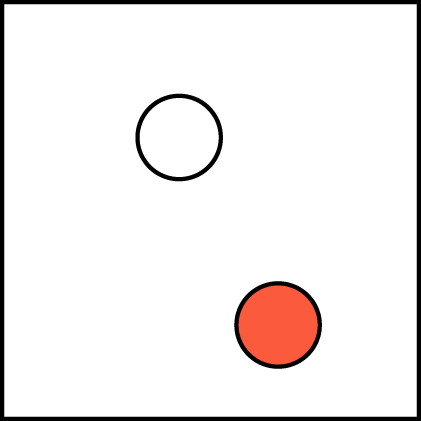
\includegraphics[width=1.5in]{sample}
%   \caption{Sample illustration.}
%   \label{fig:sampleimage}
% \end{figure}
\nocite{*}
\printbibliography
\end{document}
